% Options for packages loaded elsewhere
\PassOptionsToPackage{unicode}{hyperref}
\PassOptionsToPackage{hyphens}{url}
%
\documentclass[
]{article}
\title{STA 465 Homework 4}
\author{Tianyi Zhang 1005156607}
\date{11/04/2022}

\usepackage{amsmath,amssymb}
\usepackage{lmodern}
\usepackage{iftex}
\ifPDFTeX
  \usepackage[T1]{fontenc}
  \usepackage[utf8]{inputenc}
  \usepackage{textcomp} % provide euro and other symbols
\else % if luatex or xetex
  \usepackage{unicode-math}
  \defaultfontfeatures{Scale=MatchLowercase}
  \defaultfontfeatures[\rmfamily]{Ligatures=TeX,Scale=1}
\fi
% Use upquote if available, for straight quotes in verbatim environments
\IfFileExists{upquote.sty}{\usepackage{upquote}}{}
\IfFileExists{microtype.sty}{% use microtype if available
  \usepackage[]{microtype}
  \UseMicrotypeSet[protrusion]{basicmath} % disable protrusion for tt fonts
}{}
\makeatletter
\@ifundefined{KOMAClassName}{% if non-KOMA class
  \IfFileExists{parskip.sty}{%
    \usepackage{parskip}
  }{% else
    \setlength{\parindent}{0pt}
    \setlength{\parskip}{6pt plus 2pt minus 1pt}}
}{% if KOMA class
  \KOMAoptions{parskip=half}}
\makeatother
\usepackage{xcolor}
\IfFileExists{xurl.sty}{\usepackage{xurl}}{} % add URL line breaks if available
\IfFileExists{bookmark.sty}{\usepackage{bookmark}}{\usepackage{hyperref}}
\hypersetup{
  pdftitle={STA 465 Homework 4},
  pdfauthor={Tianyi Zhang 1005156607},
  hidelinks,
  pdfcreator={LaTeX via pandoc}}
\urlstyle{same} % disable monospaced font for URLs
\usepackage[margin=1in]{geometry}
\usepackage{color}
\usepackage{fancyvrb}
\newcommand{\VerbBar}{|}
\newcommand{\VERB}{\Verb[commandchars=\\\{\}]}
\DefineVerbatimEnvironment{Highlighting}{Verbatim}{commandchars=\\\{\}}
% Add ',fontsize=\small' for more characters per line
\usepackage{framed}
\definecolor{shadecolor}{RGB}{248,248,248}
\newenvironment{Shaded}{\begin{snugshade}}{\end{snugshade}}
\newcommand{\AlertTok}[1]{\textcolor[rgb]{0.94,0.16,0.16}{#1}}
\newcommand{\AnnotationTok}[1]{\textcolor[rgb]{0.56,0.35,0.01}{\textbf{\textit{#1}}}}
\newcommand{\AttributeTok}[1]{\textcolor[rgb]{0.77,0.63,0.00}{#1}}
\newcommand{\BaseNTok}[1]{\textcolor[rgb]{0.00,0.00,0.81}{#1}}
\newcommand{\BuiltInTok}[1]{#1}
\newcommand{\CharTok}[1]{\textcolor[rgb]{0.31,0.60,0.02}{#1}}
\newcommand{\CommentTok}[1]{\textcolor[rgb]{0.56,0.35,0.01}{\textit{#1}}}
\newcommand{\CommentVarTok}[1]{\textcolor[rgb]{0.56,0.35,0.01}{\textbf{\textit{#1}}}}
\newcommand{\ConstantTok}[1]{\textcolor[rgb]{0.00,0.00,0.00}{#1}}
\newcommand{\ControlFlowTok}[1]{\textcolor[rgb]{0.13,0.29,0.53}{\textbf{#1}}}
\newcommand{\DataTypeTok}[1]{\textcolor[rgb]{0.13,0.29,0.53}{#1}}
\newcommand{\DecValTok}[1]{\textcolor[rgb]{0.00,0.00,0.81}{#1}}
\newcommand{\DocumentationTok}[1]{\textcolor[rgb]{0.56,0.35,0.01}{\textbf{\textit{#1}}}}
\newcommand{\ErrorTok}[1]{\textcolor[rgb]{0.64,0.00,0.00}{\textbf{#1}}}
\newcommand{\ExtensionTok}[1]{#1}
\newcommand{\FloatTok}[1]{\textcolor[rgb]{0.00,0.00,0.81}{#1}}
\newcommand{\FunctionTok}[1]{\textcolor[rgb]{0.00,0.00,0.00}{#1}}
\newcommand{\ImportTok}[1]{#1}
\newcommand{\InformationTok}[1]{\textcolor[rgb]{0.56,0.35,0.01}{\textbf{\textit{#1}}}}
\newcommand{\KeywordTok}[1]{\textcolor[rgb]{0.13,0.29,0.53}{\textbf{#1}}}
\newcommand{\NormalTok}[1]{#1}
\newcommand{\OperatorTok}[1]{\textcolor[rgb]{0.81,0.36,0.00}{\textbf{#1}}}
\newcommand{\OtherTok}[1]{\textcolor[rgb]{0.56,0.35,0.01}{#1}}
\newcommand{\PreprocessorTok}[1]{\textcolor[rgb]{0.56,0.35,0.01}{\textit{#1}}}
\newcommand{\RegionMarkerTok}[1]{#1}
\newcommand{\SpecialCharTok}[1]{\textcolor[rgb]{0.00,0.00,0.00}{#1}}
\newcommand{\SpecialStringTok}[1]{\textcolor[rgb]{0.31,0.60,0.02}{#1}}
\newcommand{\StringTok}[1]{\textcolor[rgb]{0.31,0.60,0.02}{#1}}
\newcommand{\VariableTok}[1]{\textcolor[rgb]{0.00,0.00,0.00}{#1}}
\newcommand{\VerbatimStringTok}[1]{\textcolor[rgb]{0.31,0.60,0.02}{#1}}
\newcommand{\WarningTok}[1]{\textcolor[rgb]{0.56,0.35,0.01}{\textbf{\textit{#1}}}}
\usepackage{graphicx}
\makeatletter
\def\maxwidth{\ifdim\Gin@nat@width>\linewidth\linewidth\else\Gin@nat@width\fi}
\def\maxheight{\ifdim\Gin@nat@height>\textheight\textheight\else\Gin@nat@height\fi}
\makeatother
% Scale images if necessary, so that they will not overflow the page
% margins by default, and it is still possible to overwrite the defaults
% using explicit options in \includegraphics[width, height, ...]{}
\setkeys{Gin}{width=\maxwidth,height=\maxheight,keepaspectratio}
% Set default figure placement to htbp
\makeatletter
\def\fps@figure{htbp}
\makeatother
\setlength{\emergencystretch}{3em} % prevent overfull lines
\providecommand{\tightlist}{%
  \setlength{\itemsep}{0pt}\setlength{\parskip}{0pt}}
\setcounter{secnumdepth}{-\maxdimen} % remove section numbering
\usepackage{booktabs}
\usepackage{longtable}
\usepackage{array}
\usepackage{multirow}
\usepackage{wrapfig}
\usepackage{float}
\usepackage{colortbl}
\usepackage{pdflscape}
\usepackage{tabu}
\usepackage{threeparttable}
\usepackage{threeparttablex}
\usepackage[normalem]{ulem}
\usepackage{makecell}
\usepackage{xcolor}
\ifLuaTeX
  \usepackage{selnolig}  % disable illegal ligatures
\fi

\begin{document}
\maketitle

\hypertarget{question-1-sloths-in-costa-rica}{%
\section{Question 1: Sloths in Costa
Rica}\label{question-1-sloths-in-costa-rica}}

\hypertarget{question-1.1}{%
\subsection{Question 1.1}\label{question-1.1}}

\begin{Shaded}
\begin{Highlighting}[]
\NormalTok{grid}
\end{Highlighting}
\end{Shaded}

\begin{verbatim}
## class       : SpatialPolygonsDataFrame 
## features    : 511 
## extent      : -85.90801, -82.60801, 8.089453, 11.18945  (xmin, xmax, ymin, ymax)
## crs         : +proj=longlat +datum=WGS84 +no_defs +ellps=WGS84 +towgs84=0,0,0 
## variables   : 6
## names       : layer,   id,  Y, cellarea,    cov,  id2 
## min values  :     0,    3,  0,     0.01,     78,    3 
## max values  :    96, 1021, 96,     0.01, 223.25, 1021
\end{verbatim}

Looking at the \texttt{grid} dataset, we can see that it is of the
SpatialPolygonsDataFrame class and its CRS is WGS84.

\hypertarget{question-1.2}{%
\subsection{Question 1.2}\label{question-1.2}}

\begin{Shaded}
\begin{Highlighting}[]
\CommentTok{\# Model 1; Weakly Informative Priors}
\CommentTok{\# default values for priors for an rw2d and iid model are }
\CommentTok{\# both log{-}gamma(1, 0.00005)}
\NormalTok{prior.weakly }\OtherTok{\textless{}{-}} \FunctionTok{list}\NormalTok{(}\AttributeTok{prec =} \FunctionTok{list}\NormalTok{(}\AttributeTok{prior =} \StringTok{"normal"}\NormalTok{,}
                               \AttributeTok{param =} \FunctionTok{c}\NormalTok{(}\DecValTok{1}\NormalTok{, }\FloatTok{0.01}\NormalTok{)))}

\NormalTok{formula }\OtherTok{\textless{}{-}}\NormalTok{ Y }\SpecialCharTok{\textasciitilde{}} \DecValTok{1} \SpecialCharTok{+}\NormalTok{ cov }\SpecialCharTok{+}
  \FunctionTok{f}\NormalTok{(id, }\AttributeTok{model=}\StringTok{"rw2d"}\NormalTok{, }\AttributeTok{nrow =}\NormalTok{ nrow, }\AttributeTok{ncol =}\NormalTok{ ncol, }\AttributeTok{hyper =}\NormalTok{ prior.weakly) }\SpecialCharTok{+}
  \FunctionTok{f}\NormalTok{(id2, }\AttributeTok{model=}\StringTok{"iid"}\NormalTok{, }\AttributeTok{hyper =}\NormalTok{ prior.weakly)}
\NormalTok{res }\OtherTok{\textless{}{-}} \FunctionTok{inla}\NormalTok{(formula, }\AttributeTok{family =} \StringTok{"poisson"}\NormalTok{, }\AttributeTok{data =}\NormalTok{ grid}\SpecialCharTok{@}\NormalTok{data,}
    \AttributeTok{E =}\NormalTok{ cellarea, }\AttributeTok{control.predictor =} \FunctionTok{list}\NormalTok{(}\AttributeTok{compute =} \ConstantTok{TRUE}\NormalTok{))}

\FunctionTok{summary}\NormalTok{(res)}
\end{Highlighting}
\end{Shaded}

\begin{verbatim}
## 
## Call:
##    c("inla.core(formula = formula, family = family, contrasts = contrasts, 
##    ", " data = data, quantiles = quantiles, E = E, offset = offset, ", " 
##    scale = scale, weights = weights, Ntrials = Ntrials, strata = strata, 
##    ", " lp.scale = lp.scale, link.covariates = link.covariates, verbose = 
##    verbose, ", " lincomb = lincomb, selection = selection, control.compute 
##    = control.compute, ", " control.predictor = control.predictor, 
##    control.family = control.family, ", " control.inla = control.inla, 
##    control.fixed = control.fixed, ", " control.mode = control.mode, 
##    control.expert = control.expert, ", " control.hazard = control.hazard, 
##    control.lincomb = control.lincomb, ", " control.update = 
##    control.update, control.lp.scale = control.lp.scale, ", " 
##    control.pardiso = control.pardiso, only.hyperparam = only.hyperparam, 
##    ", " inla.call = inla.call, inla.arg = inla.arg, num.threads = 
##    num.threads, ", " blas.num.threads = blas.num.threads, keep = keep, 
##    working.directory = working.directory, ", " silent = silent, inla.mode 
##    = inla.mode, safe = FALSE, debug = debug, ", " .parent.frame = 
##    .parent.frame)") 
## Time used:
##     Pre = 0.976, Running = 14.2, Post = 0.0728, Total = 15.3 
## Fixed effects:
##               mean    sd 0.025quant 0.5quant 0.975quant   mode kld
## (Intercept) -2.789 1.499     -5.899   -2.732     -0.006 -2.619   0
## cov          0.021 0.007      0.008    0.021      0.035  0.021   0
## 
## Random effects:
##   Name     Model
##     id Random walk 2D
##    id2 IID model
## 
## Model hyperparameters:
##                    mean    sd 0.025quant 0.5quant 0.975quant  mode
## Precision for id  0.346 0.173      0.126    0.308      0.786 0.246
## Precision for id2 0.235 0.053      0.146    0.230      0.354 0.221
## 
## Marginal log-Likelihood:  -1639.59 
## Posterior summaries for the linear predictor and the fitted values are computed
## (Posterior marginals needs also 'control.compute=list(return.marginals.predictor=TRUE)')
\end{verbatim}

\begin{Shaded}
\begin{Highlighting}[]
\CommentTok{\#Organize Results in a Table}
\NormalTok{cred.int }\OtherTok{\textless{}{-}} \FunctionTok{data.frame}\NormalTok{(}\AttributeTok{LowerBound =}\NormalTok{ res}\SpecialCharTok{$}\NormalTok{summary.fixed}\SpecialCharTok{$}\StringTok{\textasciigrave{}}\AttributeTok{0.025quant}\StringTok{\textasciigrave{}}\NormalTok{,}
                       \AttributeTok{UpperBound =}\NormalTok{ res}\SpecialCharTok{$}\NormalTok{summary.fixed}\SpecialCharTok{$}\StringTok{\textasciigrave{}}\AttributeTok{0.975quant}\StringTok{\textasciigrave{}}\NormalTok{,}
                       \AttributeTok{Estimate =}\NormalTok{ res}\SpecialCharTok{$}\NormalTok{summary.fixed}\SpecialCharTok{$}\NormalTok{mean)}
\FunctionTok{rownames}\NormalTok{(cred.int)}\OtherTok{\textless{}{-}} \FunctionTok{c}\NormalTok{(}\StringTok{"Intercept"}\NormalTok{,}\StringTok{"Covariate"}\NormalTok{)}
\NormalTok{cred.int }\SpecialCharTok{\%\textgreater{}\%}
  \FunctionTok{kable}\NormalTok{(}
    \AttributeTok{caption =} \StringTok{"95\% Credible Intervals For Parameter Estimates,}
\StringTok{      Weakly Informative Prior"}\NormalTok{,}
    \AttributeTok{col.names =} \FunctionTok{c}\NormalTok{(}\StringTok{"Lower Bound"}\NormalTok{, }\StringTok{"Upper Bound"}\NormalTok{, }\StringTok{"Estimate"}\NormalTok{),}
    \AttributeTok{row.names =} \ConstantTok{TRUE}\NormalTok{,}
    \AttributeTok{digits =} \DecValTok{4}\NormalTok{,}
    \AttributeTok{booktabs =} \ConstantTok{TRUE}
\NormalTok{  )}
\end{Highlighting}
\end{Shaded}

\begin{table}

\caption{\label{tab:unnamed-chunk-2}95% Credible Intervals For Parameter Estimates,
      Weakly Informative Prior}
\centering
\begin{tabular}[t]{lrrr}
\toprule
  & Lower Bound & Upper Bound & Estimate\\
\midrule
Intercept & -5.8992 & -0.0058 & -2.7892\\
Covariate & 0.0081 & 0.0350 & 0.0211\\
\bottomrule
\end{tabular}
\end{table}

\begin{Shaded}
\begin{Highlighting}[]
\CommentTok{\# Model 2; Non{-}Informative Priors}
\NormalTok{prior.non }\OtherTok{\textless{}{-}} \FunctionTok{list}\NormalTok{(}\AttributeTok{prec =} \FunctionTok{list}\NormalTok{(}\AttributeTok{prior =} \StringTok{"loggamma"}\NormalTok{,}
                               \AttributeTok{param =} \FunctionTok{c}\NormalTok{(}\DecValTok{1}\NormalTok{, }\FloatTok{0.00001}\NormalTok{)))}

\NormalTok{formula }\OtherTok{\textless{}{-}}\NormalTok{ Y }\SpecialCharTok{\textasciitilde{}} \DecValTok{1} \SpecialCharTok{+}\NormalTok{ cov }\SpecialCharTok{+}
  \FunctionTok{f}\NormalTok{(id, }\AttributeTok{model=}\StringTok{"rw2d"}\NormalTok{, }\AttributeTok{nrow =}\NormalTok{ nrow, }\AttributeTok{ncol =}\NormalTok{ ncol, }\AttributeTok{hyper =}\NormalTok{ prior.non) }\SpecialCharTok{+}
  \FunctionTok{f}\NormalTok{(id2, }\AttributeTok{model=}\StringTok{"iid"}\NormalTok{, }\AttributeTok{hyper =}\NormalTok{ prior.non)}
\NormalTok{res2 }\OtherTok{\textless{}{-}} \FunctionTok{inla}\NormalTok{(formula, }\AttributeTok{family =} \StringTok{"poisson"}\NormalTok{, }\AttributeTok{data =}\NormalTok{ grid}\SpecialCharTok{@}\NormalTok{data,}
    \AttributeTok{E =}\NormalTok{ cellarea, }\AttributeTok{control.predictor =} \FunctionTok{list}\NormalTok{(}\AttributeTok{compute =} \ConstantTok{TRUE}\NormalTok{))}

\FunctionTok{summary}\NormalTok{(res2)}
\end{Highlighting}
\end{Shaded}

\begin{verbatim}
## 
## Call:
##    c("inla.core(formula = formula, family = family, contrasts = contrasts, 
##    ", " data = data, quantiles = quantiles, E = E, offset = offset, ", " 
##    scale = scale, weights = weights, Ntrials = Ntrials, strata = strata, 
##    ", " lp.scale = lp.scale, link.covariates = link.covariates, verbose = 
##    verbose, ", " lincomb = lincomb, selection = selection, control.compute 
##    = control.compute, ", " control.predictor = control.predictor, 
##    control.family = control.family, ", " control.inla = control.inla, 
##    control.fixed = control.fixed, ", " control.mode = control.mode, 
##    control.expert = control.expert, ", " control.hazard = control.hazard, 
##    control.lincomb = control.lincomb, ", " control.update = 
##    control.update, control.lp.scale = control.lp.scale, ", " 
##    control.pardiso = control.pardiso, only.hyperparam = only.hyperparam, 
##    ", " inla.call = inla.call, inla.arg = inla.arg, num.threads = 
##    num.threads, ", " blas.num.threads = blas.num.threads, keep = keep, 
##    working.directory = working.directory, ", " silent = silent, inla.mode 
##    = inla.mode, safe = FALSE, debug = debug, ", " .parent.frame = 
##    .parent.frame)") 
## Time used:
##     Pre = 0.508, Running = 15.3, Post = 0.0728, Total = 15.9 
## Fixed effects:
##               mean    sd 0.025quant 0.5quant 0.975quant   mode kld
## (Intercept) -2.566 1.426     -5.526   -2.510      0.076 -2.399   0
## cov          0.021 0.007      0.008    0.021      0.034  0.020   0
## 
## Random effects:
##   Name     Model
##     id Random walk 2D
##    id2 IID model
## 
## Model hyperparameters:
##                    mean    sd 0.025quant 0.5quant 0.975quant  mode
## Precision for id  0.464 0.268      0.152    0.398      1.159 0.300
## Precision for id2 0.236 0.053      0.146    0.231      0.354 0.222
## 
## Marginal log-Likelihood:  -1658.67 
## Posterior summaries for the linear predictor and the fitted values are computed
## (Posterior marginals needs also 'control.compute=list(return.marginals.predictor=TRUE)')
\end{verbatim}

\begin{Shaded}
\begin{Highlighting}[]
\CommentTok{\#Organize Results in a Table}
\NormalTok{cred.int2 }\OtherTok{\textless{}{-}} \FunctionTok{data.frame}\NormalTok{(}\AttributeTok{LowerBound =}\NormalTok{ res2}\SpecialCharTok{$}\NormalTok{summary.fixed}\SpecialCharTok{$}\StringTok{\textasciigrave{}}\AttributeTok{0.025quant}\StringTok{\textasciigrave{}}\NormalTok{,}
                       \AttributeTok{UpperBound =}\NormalTok{ res2}\SpecialCharTok{$}\NormalTok{summary.fixed}\SpecialCharTok{$}\StringTok{\textasciigrave{}}\AttributeTok{0.975quant}\StringTok{\textasciigrave{}}\NormalTok{,}
                       \AttributeTok{Estimate =}\NormalTok{ res2}\SpecialCharTok{$}\NormalTok{summary.fixed}\SpecialCharTok{$}\NormalTok{mean)}
\FunctionTok{rownames}\NormalTok{(cred.int2)}\OtherTok{\textless{}{-}} \FunctionTok{c}\NormalTok{(}\StringTok{"Intercept"}\NormalTok{,}\StringTok{"Covariate"}\NormalTok{)}
\NormalTok{cred.int2 }\SpecialCharTok{\%\textgreater{}\%}
  \FunctionTok{kable}\NormalTok{(}
    \AttributeTok{caption =} \StringTok{"95\% Credible Intervals For Parameter Estimates,}
\StringTok{      Non{-}Informative Prior"}\NormalTok{,}
    \AttributeTok{col.names =} \FunctionTok{c}\NormalTok{(}\StringTok{"Lower Bound"}\NormalTok{, }\StringTok{"Upper Bound"}\NormalTok{, }\StringTok{"Estimate"}\NormalTok{),}
    \AttributeTok{row.names =} \ConstantTok{TRUE}\NormalTok{,}
    \AttributeTok{digits =} \DecValTok{4}\NormalTok{,}
    \AttributeTok{booktabs =} \ConstantTok{TRUE}
\NormalTok{  )}
\end{Highlighting}
\end{Shaded}

\begin{table}

\caption{\label{tab:unnamed-chunk-3}95% Credible Intervals For Parameter Estimates,
      Non-Informative Prior}
\centering
\begin{tabular}[t]{lrrr}
\toprule
  & Lower Bound & Upper Bound & Estimate\\
\midrule
Intercept & -5.5263 & 0.0765 & -2.5658\\
Covariate & 0.0082 & 0.0340 & 0.0207\\
\bottomrule
\end{tabular}
\end{table}

The tables show that the estimates and the 95\% credible intervals for
covariates in the weakly and non-informative priors are very similar.
The 95\% credible intervals and the estimates for the intercept in the
model with weakly-informative prior is slightly lower in general.

\hypertarget{quesiton-1.3}{%
\subsection{Quesiton 1.3}\label{quesiton-1.3}}

\hypertarget{weakly-informative-model}{%
\subsubsection{Weakly Informative
Model}\label{weakly-informative-model}}

The following maps are for the weakly informative model.

\begin{Shaded}
\begin{Highlighting}[]
\DocumentationTok{\#\#\#\# Create maps of the random effects \#\#\#\#}
\CommentTok{\# Weakly informative model}
\NormalTok{grid}\SpecialCharTok{$}\NormalTok{respa }\OtherTok{\textless{}{-}}\NormalTok{ res}\SpecialCharTok{$}\NormalTok{summary.random}\SpecialCharTok{$}\NormalTok{id[grid}\SpecialCharTok{$}\NormalTok{id, }\StringTok{"mean"}\NormalTok{]}
\NormalTok{grid}\SpecialCharTok{$}\NormalTok{reiid }\OtherTok{\textless{}{-}}\NormalTok{ res}\SpecialCharTok{$}\NormalTok{summary.random}\SpecialCharTok{$}\NormalTok{id2[, }\StringTok{"mean"}\NormalTok{]}

\FunctionTok{tm\_shape}\NormalTok{(grid) }\SpecialCharTok{+}
  \FunctionTok{tm\_polygons}\NormalTok{(}\AttributeTok{col =} \FunctionTok{c}\NormalTok{(}\StringTok{"respa"}\NormalTok{, }\StringTok{"reiid"}\NormalTok{), }\AttributeTok{style =} \StringTok{"cont"}\NormalTok{, }\AttributeTok{border.col =} \StringTok{"transparent"}\NormalTok{)  }\SpecialCharTok{+}
  \FunctionTok{tm\_shape}\NormalTok{(gridborder) }\SpecialCharTok{+} \FunctionTok{tm\_borders}\NormalTok{() }\SpecialCharTok{+}
  \FunctionTok{tm\_facets}\NormalTok{(}\AttributeTok{ncol =} \DecValTok{2}\NormalTok{) }\SpecialCharTok{+} \FunctionTok{tm\_legend}\NormalTok{(}\AttributeTok{legend.position =} \FunctionTok{c}\NormalTok{(}\StringTok{"left"}\NormalTok{, }\StringTok{"bottom"}\NormalTok{))}
\end{Highlighting}
\end{Shaded}

\begin{verbatim}
## Variable(s) "respa" contains positive and negative values, so midpoint is set to 0. Set midpoint = NA to show the full spectrum of the color palette.
\end{verbatim}

\begin{verbatim}
## Variable(s) "reiid" contains positive and negative values, so midpoint is set to 0. Set midpoint = NA to show the full spectrum of the color palette.
\end{verbatim}

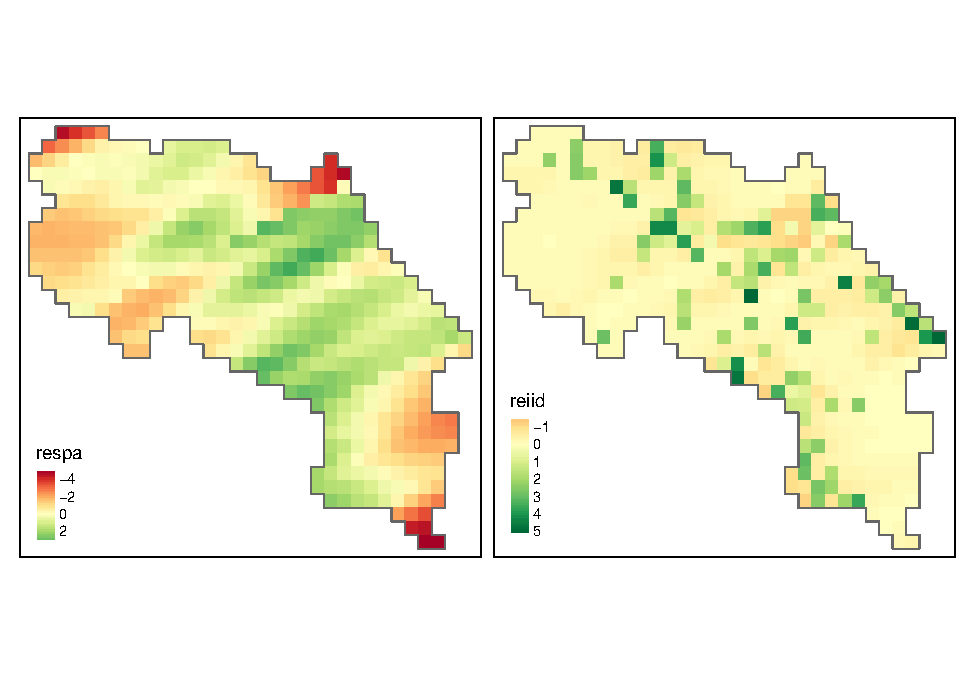
\includegraphics{hw4_files/figure-latex/unnamed-chunk-4-1.pdf}

\begin{Shaded}
\begin{Highlighting}[]
\CommentTok{\# Predicted counts per cell}
\NormalTok{cellarea }\OtherTok{\textless{}{-}}\NormalTok{ resolution}\SpecialCharTok{*}\NormalTok{resolution}
\NormalTok{grid}\SpecialCharTok{$}\NormalTok{NE }\OtherTok{\textless{}{-}}\NormalTok{ res}\SpecialCharTok{$}\NormalTok{summary.fitted.values[, }\StringTok{"mean"}\NormalTok{] }\SpecialCharTok{*}\NormalTok{ cellarea}
\NormalTok{grid}\SpecialCharTok{$}\NormalTok{LL }\OtherTok{\textless{}{-}}\NormalTok{ res}\SpecialCharTok{$}\NormalTok{summary.fitted.values[, }\StringTok{"0.025quant"}\NormalTok{] }\SpecialCharTok{*}\NormalTok{ cellarea}
\NormalTok{grid}\SpecialCharTok{$}\NormalTok{UL }\OtherTok{\textless{}{-}}\NormalTok{ res}\SpecialCharTok{$}\NormalTok{summary.fitted.values[, }\StringTok{"0.975quant"}\NormalTok{] }\SpecialCharTok{*}\NormalTok{ cellarea}
\CommentTok{\#summary(grid)}

\CommentTok{\# Create maps for the predicted counts, its lower interval, and its upper}
\CommentTok{\# interval respectively}
\CommentTok{\# NE: map of predicted counts}
\CommentTok{\# LL: map of lower limit}
\CommentTok{\# UL: map of upper limit}
\FunctionTok{tm\_shape}\NormalTok{(grid) }\SpecialCharTok{+}
  \FunctionTok{tm\_polygons}\NormalTok{(}\AttributeTok{col =} \FunctionTok{c}\NormalTok{(}\StringTok{"NE"}\NormalTok{, }\StringTok{"LL"}\NormalTok{, }\StringTok{"UL"}\NormalTok{),}
              \AttributeTok{style =} \StringTok{\textquotesingle{}fixed\textquotesingle{}}\NormalTok{, }\AttributeTok{border.col =} \StringTok{"transparent"}\NormalTok{,}
              \AttributeTok{breaks =} \FunctionTok{c}\NormalTok{(}\DecValTok{0}\NormalTok{, }\DecValTok{10}\NormalTok{, }\DecValTok{50}\NormalTok{, }\DecValTok{100}\NormalTok{, }\FunctionTok{ceiling}\NormalTok{(}\FunctionTok{max}\NormalTok{(grid}\SpecialCharTok{$}\NormalTok{UL)))) }\SpecialCharTok{+}
  \FunctionTok{tm\_shape}\NormalTok{(gridborder) }\SpecialCharTok{+} \FunctionTok{tm\_borders}\NormalTok{() }\SpecialCharTok{+}
  \FunctionTok{tm\_facets}\NormalTok{(}\AttributeTok{ncol =} \DecValTok{3}\NormalTok{) }\SpecialCharTok{+} \FunctionTok{tm\_legend}\NormalTok{(}\AttributeTok{legend.position =} \FunctionTok{c}\NormalTok{(}\StringTok{"left"}\NormalTok{, }\StringTok{"bottom"}\NormalTok{)) }
\end{Highlighting}
\end{Shaded}

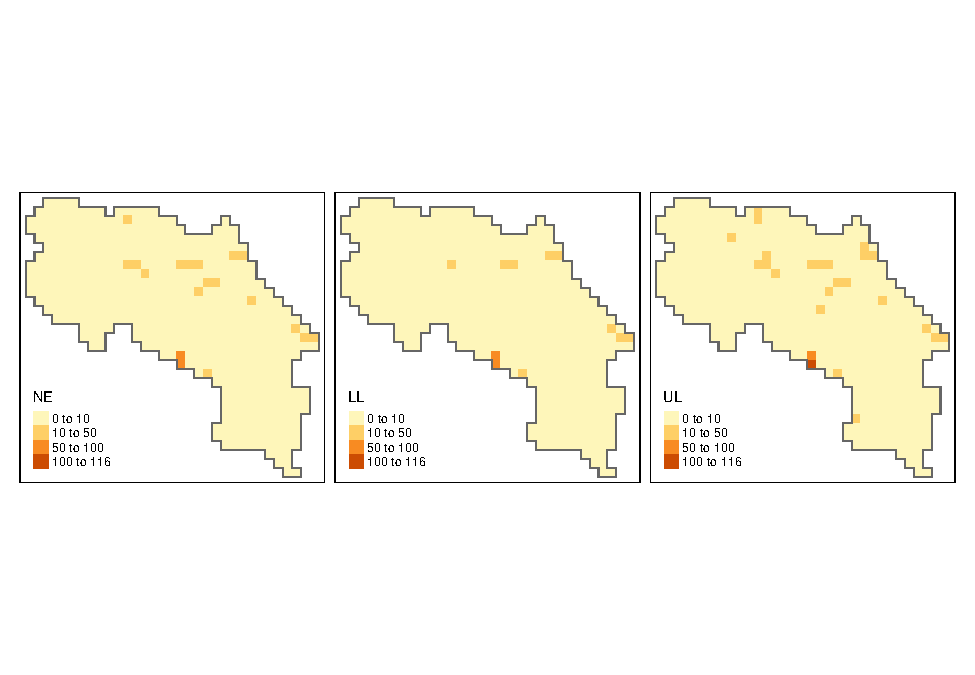
\includegraphics{hw4_files/figure-latex/unnamed-chunk-4-2.pdf}

The first two maps are maps of the random effects, rw2d and iid,
respectively.

The next set of three maps are maps of the predicted counts per cell,
its 95\% lower limit and its upper limit, respectively.

\hypertarget{non-informative-model}{%
\subsubsection{Non-Informative Model}\label{non-informative-model}}

The following maps are for the non-informative model.

\begin{Shaded}
\begin{Highlighting}[]
\DocumentationTok{\#\#\#\# Create maps of the random effects \#\#\#\#}
\CommentTok{\# Non{-}informative model}
\NormalTok{grid}\SpecialCharTok{$}\NormalTok{respa }\OtherTok{\textless{}{-}}\NormalTok{ res2}\SpecialCharTok{$}\NormalTok{summary.random}\SpecialCharTok{$}\NormalTok{id[grid}\SpecialCharTok{$}\NormalTok{id, }\StringTok{"mean"}\NormalTok{]}
\NormalTok{grid}\SpecialCharTok{$}\NormalTok{reiid }\OtherTok{\textless{}{-}}\NormalTok{ res2}\SpecialCharTok{$}\NormalTok{summary.random}\SpecialCharTok{$}\NormalTok{id2[, }\StringTok{"mean"}\NormalTok{]}

\FunctionTok{tm\_shape}\NormalTok{(grid) }\SpecialCharTok{+}
  \FunctionTok{tm\_polygons}\NormalTok{(}\AttributeTok{col =} \FunctionTok{c}\NormalTok{(}\StringTok{"respa"}\NormalTok{, }\StringTok{"reiid"}\NormalTok{), }\AttributeTok{style =} \StringTok{"cont"}\NormalTok{, }\AttributeTok{border.col =} \StringTok{"transparent"}\NormalTok{)  }\SpecialCharTok{+}
  \FunctionTok{tm\_shape}\NormalTok{(gridborder) }\SpecialCharTok{+} \FunctionTok{tm\_borders}\NormalTok{() }\SpecialCharTok{+}
  \FunctionTok{tm\_facets}\NormalTok{(}\AttributeTok{ncol =} \DecValTok{2}\NormalTok{) }\SpecialCharTok{+} \FunctionTok{tm\_legend}\NormalTok{(}\AttributeTok{legend.position =} \FunctionTok{c}\NormalTok{(}\StringTok{"left"}\NormalTok{, }\StringTok{"bottom"}\NormalTok{))}
\end{Highlighting}
\end{Shaded}

\begin{verbatim}
## Variable(s) "respa" contains positive and negative values, so midpoint is set to 0. Set midpoint = NA to show the full spectrum of the color palette.
\end{verbatim}

\begin{verbatim}
## Variable(s) "reiid" contains positive and negative values, so midpoint is set to 0. Set midpoint = NA to show the full spectrum of the color palette.
\end{verbatim}

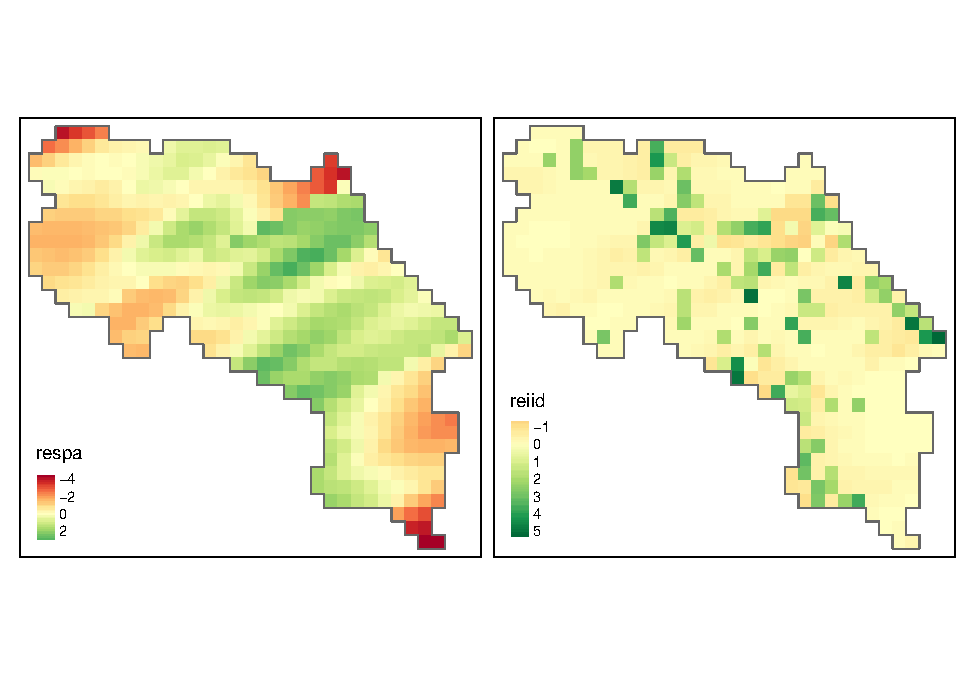
\includegraphics{hw4_files/figure-latex/unnamed-chunk-5-1.pdf}

\begin{Shaded}
\begin{Highlighting}[]
\CommentTok{\# Predicted counts per cell}
\NormalTok{cellarea }\OtherTok{\textless{}{-}}\NormalTok{ resolution}\SpecialCharTok{*}\NormalTok{resolution}
\NormalTok{grid}\SpecialCharTok{$}\NormalTok{NE }\OtherTok{\textless{}{-}}\NormalTok{ res2}\SpecialCharTok{$}\NormalTok{summary.fitted.values[, }\StringTok{"mean"}\NormalTok{] }\SpecialCharTok{*}\NormalTok{ cellarea}
\NormalTok{grid}\SpecialCharTok{$}\NormalTok{LL }\OtherTok{\textless{}{-}}\NormalTok{ res2}\SpecialCharTok{$}\NormalTok{summary.fitted.values[, }\StringTok{"0.025quant"}\NormalTok{] }\SpecialCharTok{*}\NormalTok{ cellarea}
\NormalTok{grid}\SpecialCharTok{$}\NormalTok{UL }\OtherTok{\textless{}{-}}\NormalTok{ res2}\SpecialCharTok{$}\NormalTok{summary.fitted.values[, }\StringTok{"0.975quant"}\NormalTok{] }\SpecialCharTok{*}\NormalTok{ cellarea}
\CommentTok{\#summary(grid)}

\CommentTok{\# Create maps for the predicted counts, its lower interval, and its upper}
\CommentTok{\# interval respectively}
\CommentTok{\# NE: map of predicted counts}
\CommentTok{\# LL: map of lower limit}
\CommentTok{\# UL: map of upper limit}
\FunctionTok{tm\_shape}\NormalTok{(grid) }\SpecialCharTok{+}
  \FunctionTok{tm\_polygons}\NormalTok{(}\AttributeTok{col =} \FunctionTok{c}\NormalTok{(}\StringTok{"NE"}\NormalTok{, }\StringTok{"LL"}\NormalTok{, }\StringTok{"UL"}\NormalTok{),}
              \AttributeTok{style =} \StringTok{\textquotesingle{}fixed\textquotesingle{}}\NormalTok{, }\AttributeTok{border.col =} \StringTok{"transparent"}\NormalTok{,}
              \AttributeTok{breaks =} \FunctionTok{c}\NormalTok{(}\DecValTok{0}\NormalTok{, }\DecValTok{10}\NormalTok{, }\DecValTok{50}\NormalTok{, }\DecValTok{100}\NormalTok{, }\FunctionTok{ceiling}\NormalTok{(}\FunctionTok{max}\NormalTok{(grid}\SpecialCharTok{$}\NormalTok{UL)))) }\SpecialCharTok{+}
  \FunctionTok{tm\_shape}\NormalTok{(gridborder) }\SpecialCharTok{+} \FunctionTok{tm\_borders}\NormalTok{() }\SpecialCharTok{+}
  \FunctionTok{tm\_facets}\NormalTok{(}\AttributeTok{ncol =} \DecValTok{3}\NormalTok{) }\SpecialCharTok{+} \FunctionTok{tm\_legend}\NormalTok{(}\AttributeTok{legend.position =} \FunctionTok{c}\NormalTok{(}\StringTok{"left"}\NormalTok{, }\StringTok{"bottom"}\NormalTok{)) }
\end{Highlighting}
\end{Shaded}

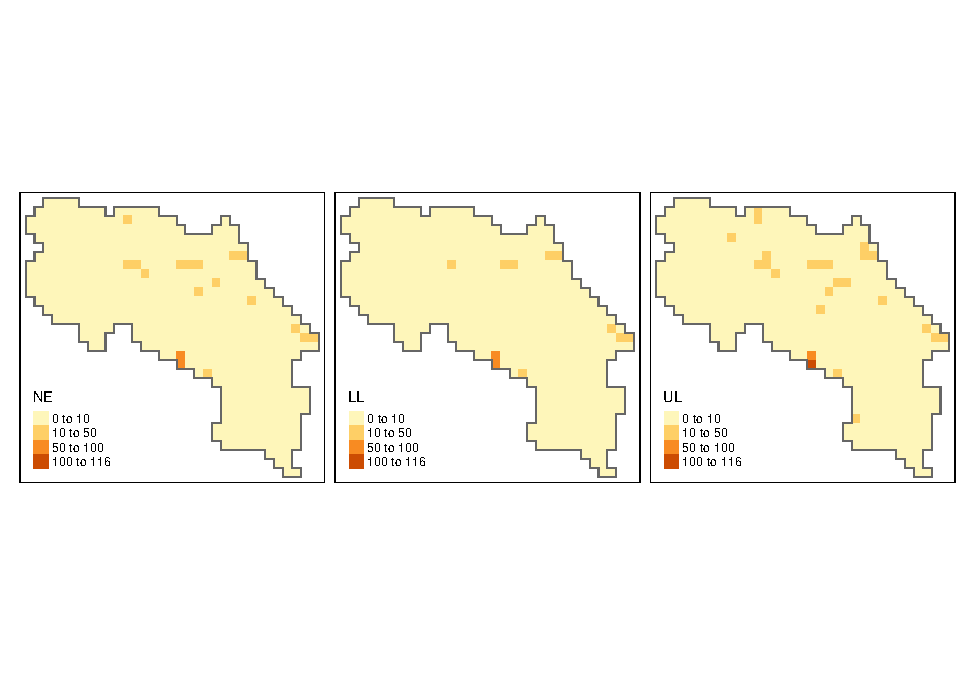
\includegraphics{hw4_files/figure-latex/unnamed-chunk-5-2.pdf}

The first two maps are maps of the random effects, rw2d and iid,
respectively.

The next set of three maps are maps of the predicted counts per cell,
its 95\% lower limit and its upper limit, respectively.

There does not seem to be any major differences in the predicted cell
counts and its 95\% credible intervals for the weakly informative prior
and non-informative prior.

\hypertarget{question-2}{%
\section{Question 2}\label{question-2}}

\hypertarget{question-2.1}{%
\subsection{Question 2.1}\label{question-2.1}}

\begin{Shaded}
\begin{Highlighting}[]
\DocumentationTok{\#\#\#\# Get data \#\#\#\#}
\CommentTok{\# Data acquisition code is from Lab 5}
\FunctionTok{library}\NormalTok{(SpatialEpi)}
\FunctionTok{library}\NormalTok{(sf)}
\end{Highlighting}
\end{Shaded}

\begin{verbatim}
## Linking to GEOS 3.9.1, GDAL 3.2.1, PROJ 7.2.1; sf_use_s2() is TRUE
\end{verbatim}

\begin{Shaded}
\begin{Highlighting}[]
\FunctionTok{library}\NormalTok{(spdep)}
\end{Highlighting}
\end{Shaded}

\begin{verbatim}
## Loading required package: spData
\end{verbatim}

\begin{Shaded}
\begin{Highlighting}[]
\FunctionTok{data}\NormalTok{(pennLC)}
\NormalTok{population }\OtherTok{\textless{}{-}}\NormalTok{ pennLC}\SpecialCharTok{$}\NormalTok{data}\SpecialCharTok{$}\NormalTok{population}
\NormalTok{cases }\OtherTok{\textless{}{-}}\NormalTok{ pennLC}\SpecialCharTok{$}\NormalTok{data}\SpecialCharTok{$}\NormalTok{cases}
\NormalTok{n.strata }\OtherTok{\textless{}{-}} \DecValTok{16}
\NormalTok{E }\OtherTok{\textless{}{-}} \FunctionTok{expected}\NormalTok{(population, cases, n.strata)}
\NormalTok{d }\OtherTok{\textless{}{-}} \FunctionTok{aggregate}\NormalTok{(}\AttributeTok{x =}\NormalTok{ pennLC}\SpecialCharTok{$}\NormalTok{data}\SpecialCharTok{$}\NormalTok{cases, }\AttributeTok{by =} \FunctionTok{list}\NormalTok{(}\AttributeTok{county =}\NormalTok{ pennLC}\SpecialCharTok{$}\NormalTok{data}\SpecialCharTok{$}\NormalTok{county), }\AttributeTok{FUN =}\NormalTok{ sum)}

\CommentTok{\# convert from spatial polygon to simple feature}
\NormalTok{pennLC.sf }\OtherTok{\textless{}{-}} \FunctionTok{st\_as\_sf}\NormalTok{(pennLC}\SpecialCharTok{$}\NormalTok{spatial.polygon)}
\NormalTok{pennLC.sf}\SpecialCharTok{$}\NormalTok{county }\OtherTok{\textless{}{-}}\NormalTok{ d}\SpecialCharTok{$}\NormalTok{county}
\NormalTok{pennLC.sf}\SpecialCharTok{$}\NormalTok{counts }\OtherTok{\textless{}{-}}\NormalTok{ d}\SpecialCharTok{$}\NormalTok{x}
\NormalTok{pennLC.sf}\SpecialCharTok{$}\NormalTok{E }\OtherTok{\textless{}{-}}\NormalTok{ E[}\FunctionTok{match}\NormalTok{(pennLC.sf}\SpecialCharTok{$}\NormalTok{county, }\FunctionTok{unique}\NormalTok{(pennLC}\SpecialCharTok{$}\NormalTok{data}\SpecialCharTok{$}\NormalTok{county))]}
\NormalTok{pennLC.sf }\OtherTok{\textless{}{-}} \FunctionTok{merge}\NormalTok{(pennLC.sf, pennLC}\SpecialCharTok{$}\NormalTok{smoking, }\AttributeTok{by.x =} \StringTok{"county"}\NormalTok{, }\AttributeTok{by.y =} \StringTok{"county"}\NormalTok{)}
\NormalTok{pennLC.sf }\OtherTok{\textless{}{-}}\NormalTok{ pennLC.sf}\SpecialCharTok{\%\textgreater{}\%}
  \FunctionTok{mutate}\NormalTok{(}\AttributeTok{SIR =}\NormalTok{ counts}\SpecialCharTok{/}\NormalTok{E)}

\DocumentationTok{\#\#\#\# Fit models \#\#\#\#}
\CommentTok{\# Using Default Priors}
\DocumentationTok{\#\#\#\#\# Complete pooling and smoking covariate (no random effect) \#\#\#\#\#}
\NormalTok{formula.}\DecValTok{2}\NormalTok{.}\FloatTok{1.1} \OtherTok{\textless{}{-}}\NormalTok{ counts }\SpecialCharTok{\textasciitilde{}} \DecValTok{1} \SpecialCharTok{+}\NormalTok{ smoking}
\NormalTok{res.}\DecValTok{2}\NormalTok{.}\FloatTok{1.1} \OtherTok{\textless{}{-}} \FunctionTok{inla}\NormalTok{(formula.}\DecValTok{2}\NormalTok{.}\FloatTok{1.1}\NormalTok{, }\AttributeTok{family =} \StringTok{"poisson"}\NormalTok{, }\AttributeTok{data =}\NormalTok{ pennLC.sf,}
            \AttributeTok{E =}\NormalTok{ pennLC.sf}\SpecialCharTok{$}\NormalTok{E, }\AttributeTok{control.predictor =} \FunctionTok{list}\NormalTok{(}\AttributeTok{compute =} \ConstantTok{TRUE}\NormalTok{),}
            \AttributeTok{control.compute =} \FunctionTok{list}\NormalTok{(}\AttributeTok{cpo=}\ConstantTok{TRUE}\NormalTok{))}

\DocumentationTok{\#\#\#\#\# Hierarchical random effect (iid) {-} (intercept only) \#\#\#\#\#}
\NormalTok{formula.}\DecValTok{2}\NormalTok{.}\FloatTok{1.2} \OtherTok{\textless{}{-}}\NormalTok{ counts }\SpecialCharTok{\textasciitilde{}} \DecValTok{1} \SpecialCharTok{+} \FunctionTok{f}\NormalTok{(county, }\AttributeTok{model =} \StringTok{"iid"}\NormalTok{)}
\NormalTok{res.}\DecValTok{2}\NormalTok{.}\FloatTok{1.2} \OtherTok{\textless{}{-}} \FunctionTok{inla}\NormalTok{(formula.}\DecValTok{2}\NormalTok{.}\FloatTok{1.2}\NormalTok{, }\AttributeTok{family =} \StringTok{"poisson"}\NormalTok{, }\AttributeTok{data =}\NormalTok{ pennLC.sf,}
            \AttributeTok{E =}\NormalTok{ pennLC.sf}\SpecialCharTok{$}\NormalTok{E, }\AttributeTok{control.predictor =} \FunctionTok{list}\NormalTok{(}\AttributeTok{compute =} \ConstantTok{TRUE}\NormalTok{),}
            \AttributeTok{control.compute =} \FunctionTok{list}\NormalTok{(}\AttributeTok{cpo=}\ConstantTok{TRUE}\NormalTok{))}

\DocumentationTok{\#\#\#\#\# Hierarchical random effect (iid) + smoking covariate \#\#\#\#\#}
\CommentTok{\# add a column of numbers (need both intercept and slope to vary)}
\NormalTok{pennLC.sf}\SpecialCharTok{$}\NormalTok{county\_dup }\OtherTok{\textless{}{-}}\NormalTok{ pennLC.sf}\SpecialCharTok{$}\NormalTok{county}
\NormalTok{formula.}\DecValTok{2}\NormalTok{.}\FloatTok{1.3} \OtherTok{\textless{}{-}}\NormalTok{ counts }\SpecialCharTok{\textasciitilde{}} \DecValTok{1} \SpecialCharTok{+}\NormalTok{ smoking }\SpecialCharTok{+} \FunctionTok{f}\NormalTok{(county, }\AttributeTok{model =} \StringTok{"iid"}\NormalTok{) }\SpecialCharTok{+}
  \FunctionTok{f}\NormalTok{(county\_dup, smoking, }\AttributeTok{model =} \StringTok{"iid"}\NormalTok{)}
\NormalTok{res.}\DecValTok{2}\NormalTok{.}\FloatTok{1.3} \OtherTok{\textless{}{-}} \FunctionTok{inla}\NormalTok{(formula.}\DecValTok{2}\NormalTok{.}\FloatTok{1.3}\NormalTok{, }\AttributeTok{family =} \StringTok{"poisson"}\NormalTok{, }\AttributeTok{data =}\NormalTok{ pennLC.sf,}
            \AttributeTok{E =}\NormalTok{ pennLC.sf}\SpecialCharTok{$}\NormalTok{E, }\AttributeTok{control.predictor =} \FunctionTok{list}\NormalTok{(}\AttributeTok{compute =} \ConstantTok{TRUE}\NormalTok{),}
            \AttributeTok{control.compute =} \FunctionTok{list}\NormalTok{(}\AttributeTok{cpo=}\ConstantTok{TRUE}\NormalTok{))}

\DocumentationTok{\#\#\#\#\# Spatial + iid random effect \#\#\#\#\#}
\CommentTok{\# use BYM for spatial random effect}
\DocumentationTok{\#\# Values of E\_i and neighborhood structure}
\NormalTok{E.penn }\OtherTok{\textless{}{-}}\NormalTok{ pennLC.sf}\SpecialCharTok{$}\NormalTok{E}
\NormalTok{neighbor.penn }\OtherTok{\textless{}{-}} \FunctionTok{poly2nb}\NormalTok{(pennLC.sf)}

\FunctionTok{nb2INLA}\NormalTok{(}\StringTok{"npenn.adj"}\NormalTok{, neighbor.penn)}
\NormalTok{g }\OtherTok{\textless{}{-}} \FunctionTok{inla.read.graph}\NormalTok{(}\AttributeTok{filename =} \StringTok{"npenn.adj"}\NormalTok{)}

\NormalTok{pennLC.sf}\SpecialCharTok{$}\NormalTok{re\_u }\OtherTok{\textless{}{-}} \DecValTok{1}\SpecialCharTok{:}\FunctionTok{nrow}\NormalTok{(pennLC.sf)}
\NormalTok{pennLC.sf}\SpecialCharTok{$}\NormalTok{re\_v }\OtherTok{\textless{}{-}} \DecValTok{1}\SpecialCharTok{:}\FunctionTok{nrow}\NormalTok{(pennLC.sf)}

\NormalTok{formula.}\DecValTok{2}\NormalTok{.}\FloatTok{1.4} \OtherTok{\textless{}{-}}\NormalTok{ counts }\SpecialCharTok{\textasciitilde{}} \DecValTok{1} \SpecialCharTok{+} \FunctionTok{f}\NormalTok{(re\_u, }\AttributeTok{model =} \StringTok{"besag"}\NormalTok{, }\AttributeTok{graph =}\NormalTok{ g) }\SpecialCharTok{+}
  \FunctionTok{f}\NormalTok{(re\_v, }\AttributeTok{model =} \StringTok{"iid"}\NormalTok{)}
\NormalTok{res.}\DecValTok{2}\NormalTok{.}\FloatTok{1.4} \OtherTok{\textless{}{-}} \FunctionTok{inla}\NormalTok{(formula.}\DecValTok{2}\NormalTok{.}\FloatTok{1.4}\NormalTok{, }\AttributeTok{family =} \StringTok{"poisson"}\NormalTok{, }\AttributeTok{data =}\NormalTok{ pennLC.sf,}
            \AttributeTok{E =}\NormalTok{ pennLC.sf}\SpecialCharTok{$}\NormalTok{E, }\AttributeTok{control.predictor =} \FunctionTok{list}\NormalTok{(}\AttributeTok{compute =} \ConstantTok{TRUE}\NormalTok{),}
            \AttributeTok{control.compute =} \FunctionTok{list}\NormalTok{(}\AttributeTok{cpo=}\ConstantTok{TRUE}\NormalTok{))}

\DocumentationTok{\#\#\#\#\# Spatial + iid random effect + smoking covariate \#\#\#\#\#}
\NormalTok{formula.}\DecValTok{2}\NormalTok{.}\FloatTok{1.5} \OtherTok{\textless{}{-}}\NormalTok{ counts }\SpecialCharTok{\textasciitilde{}}\NormalTok{ smoking }\SpecialCharTok{+} \FunctionTok{f}\NormalTok{(re\_u, }\AttributeTok{model =} \StringTok{"besag"}\NormalTok{, }\AttributeTok{graph =}\NormalTok{ g) }\SpecialCharTok{+}
  \FunctionTok{f}\NormalTok{(re\_v, }\AttributeTok{model =} \StringTok{"iid"}\NormalTok{)}
\NormalTok{res.}\DecValTok{2}\NormalTok{.}\FloatTok{1.5} \OtherTok{\textless{}{-}} \FunctionTok{inla}\NormalTok{(formula.}\DecValTok{2}\NormalTok{.}\FloatTok{1.5}\NormalTok{, }\AttributeTok{family =} \StringTok{"poisson"}\NormalTok{, }\AttributeTok{data =}\NormalTok{ pennLC.sf,}
            \AttributeTok{E =}\NormalTok{ pennLC.sf}\SpecialCharTok{$}\NormalTok{E, }\AttributeTok{control.predictor =} \FunctionTok{list}\NormalTok{(}\AttributeTok{compute =} \ConstantTok{TRUE}\NormalTok{),}
            \AttributeTok{control.compute =} \FunctionTok{list}\NormalTok{(}\AttributeTok{cpo=}\ConstantTok{TRUE}\NormalTok{))}
\end{Highlighting}
\end{Shaded}

\hypertarget{complete-pooling-and-smoking-covariate-no-random-effect}{%
\subsubsection{2.1.1: Complete pooling and smoking covariate (no random
effect)}\label{complete-pooling-and-smoking-covariate-no-random-effect}}

\begin{Shaded}
\begin{Highlighting}[]
\DocumentationTok{\#\#\#\# Make a table of CPO and PIT values \#\#\#\#}
\NormalTok{cpo.}\DecValTok{2}\NormalTok{.}\FloatTok{1.1} \OtherTok{\textless{}{-}} \FunctionTok{data.frame}\NormalTok{(}\AttributeTok{CPO =}\NormalTok{ res.}\DecValTok{2}\NormalTok{.}\FloatTok{1.1}\SpecialCharTok{$}\NormalTok{cpo}\SpecialCharTok{$}\NormalTok{cpo,}
                       \AttributeTok{PIT =}\NormalTok{ res.}\DecValTok{2}\NormalTok{.}\FloatTok{1.1}\SpecialCharTok{$}\NormalTok{cpo}\SpecialCharTok{$}\NormalTok{pit)}
\NormalTok{cpo.}\DecValTok{2}\NormalTok{.}\FloatTok{1.1} \SpecialCharTok{\%\textgreater{}\%}
  \FunctionTok{kable}\NormalTok{(}
    \AttributeTok{caption =} \StringTok{"CPO and PIT values for Complete Pooling and Smoking }
\StringTok{    Covariate (no random effect)"}\NormalTok{,}
    \AttributeTok{row.names =} \ConstantTok{TRUE}\NormalTok{,}
    \AttributeTok{digits =} \DecValTok{4}\NormalTok{,}
    \AttributeTok{booktabs =} \ConstantTok{TRUE}
\NormalTok{  )}
\end{Highlighting}
\end{Shaded}

\begin{table}

\caption{\label{tab:unnamed-chunk-7}CPO and PIT values for Complete Pooling and Smoking 
    Covariate (no random effect)}
\centering
\begin{tabular}[t]{lrr}
\toprule
  & CPO & PIT\\
\midrule
1 & 0.0113 & 0.0467\\
2 & 0.0005 & 0.9939\\
3 & 0.0023 & 0.0074\\
4 & 0.0210 & 0.2171\\
5 & 0.0394 & 0.1842\\
\addlinespace
6 & 0.0221 & 0.5737\\
7 & 0.0153 & 0.9114\\
8 & 0.0473 & 0.6924\\
9 & 0.0016 & 0.9875\\
10 & 0.0138 & 0.9077\\
\addlinespace
11 & 0.0010 & 0.0046\\
12 & 0.0974 & 0.8638\\
13 & 0.0132 & 0.0489\\
14 & 0.0103 & 0.0443\\
15 & 0.0225 & 0.5715\\
\addlinespace
16 & 0.0685 & 0.4574\\
17 & 0.0464 & 0.5551\\
18 & 0.0303 & 0.1081\\
19 & 0.0325 & 0.8555\\
20 & 0.0365 & 0.2749\\
\addlinespace
21 & 0.0014 & 0.0068\\
22 & 0.0067 & 0.0462\\
23 & 0.0016 & 0.9870\\
24 & 0.0713 & 0.5504\\
25 & 0.0252 & 0.5589\\
\addlinespace
26 & 0.0157 & 0.8952\\
27 & 0.1639 & 0.3889\\
28 & 0.0358 & 0.3719\\
29 & 0.1180 & 0.5192\\
30 & 0.0423 & 0.8482\\
\addlinespace
31 & 0.0164 & 0.0503\\
32 & 0.0457 & 0.4219\\
33 & 0.0314 & 0.1280\\
34 & 0.0005 & 0.0008\\
35 & 0.0025 & 0.0148\\
\addlinespace
36 & 0.0018 & 0.0138\\
37 & 0.0034 & 0.0140\\
38 & 0.0034 & 0.0137\\
39 & 0.0244 & 0.4490\\
40 & 0.0024 & 0.0180\\
\addlinespace
41 & 0.0284 & 0.2247\\
42 & 0.0522 & 0.2740\\
43 & 0.0051 & 0.0251\\
44 & 0.0442 & 0.8065\\
45 & 0.0201 & 0.8825\\
\addlinespace
46 & 0.0014 & 0.9838\\
47 & 0.0162 & 0.0306\\
48 & 0.0124 & 0.8934\\
49 & 0.0397 & 0.3636\\
50 & 0.0687 & 0.6518\\
\addlinespace
51 & 0.0000 & 1.0000\\
52 & 0.0525 & 0.2768\\
53 & 0.0405 & 0.9135\\
54 & 0.0167 & 0.1277\\
55 & 0.0747 & 0.5799\\
\addlinespace
56 & 0.0016 & 0.0051\\
57 & 0.0325 & 0.0487\\
58 & 0.0655 & 0.4327\\
59 & 0.0196 & 0.0644\\
60 & 0.0722 & 0.4404\\
\addlinespace
61 & 0.0059 & 0.9830\\
62 & 0.0569 & 0.3211\\
63 & 0.0243 & 0.7264\\
64 & 0.0584 & 0.6064\\
65 & 0.0112 & 0.8695\\
\addlinespace
66 & 0.0212 & 0.0512\\
67 & 0.0206 & 0.3181\\
\bottomrule
\end{tabular}
\end{table}

\begin{Shaded}
\begin{Highlighting}[]
\DocumentationTok{\#\#\#\# Create maps of predicted prevalence and its standard deviation \#\#\#\#}
\NormalTok{pennLC.sf}\SpecialCharTok{$}\NormalTok{m2.}\DecValTok{1}\NormalTok{.}\FloatTok{1.}\NormalTok{mean }\OtherTok{\textless{}{-}}\NormalTok{ res.}\DecValTok{2}\NormalTok{.}\FloatTok{1.1}\SpecialCharTok{$}\NormalTok{summary.fitted.values[,}\StringTok{"mean"}\NormalTok{]}\SpecialCharTok{*}\NormalTok{E.penn}
\NormalTok{pennLC.sf}\SpecialCharTok{$}\NormalTok{m2.}\DecValTok{1}\NormalTok{.}\FloatTok{1.}\NormalTok{sd }\OtherTok{\textless{}{-}}\NormalTok{ res.}\DecValTok{2}\NormalTok{.}\FloatTok{1.1}\SpecialCharTok{$}\NormalTok{summary.fitted.values[,}\StringTok{"sd"}\NormalTok{]}\SpecialCharTok{*}\NormalTok{E.penn}

\NormalTok{res.}\DecValTok{2}\NormalTok{.}\DecValTok{1}\NormalTok{.}\FloatTok{1.}\NormalTok{mean }\OtherTok{\textless{}{-}} \FunctionTok{tm\_shape}\NormalTok{(pennLC.sf) }\SpecialCharTok{+} 
  \FunctionTok{tm\_polygons}\NormalTok{(}\StringTok{"m2.1.1.mean"}\NormalTok{) }\SpecialCharTok{+} 
  \FunctionTok{tm\_layout}\NormalTok{(}\AttributeTok{main.title =} \StringTok{"Predicted Prevalence"}\NormalTok{)}

\NormalTok{res.}\DecValTok{2}\NormalTok{.}\DecValTok{1}\NormalTok{.}\FloatTok{1.}\NormalTok{sd }\OtherTok{\textless{}{-}} \FunctionTok{tm\_shape}\NormalTok{(pennLC.sf) }\SpecialCharTok{+} 
  \FunctionTok{tm\_polygons}\NormalTok{(}\StringTok{"m2.1.1.sd"}\NormalTok{) }\SpecialCharTok{+} 
  \FunctionTok{tm\_layout}\NormalTok{(}\AttributeTok{main.title =} \StringTok{"Standard Deviation of Predicted Prevalence"}\NormalTok{)}

\FunctionTok{tmap\_arrange}\NormalTok{(res.}\DecValTok{2}\NormalTok{.}\DecValTok{1}\NormalTok{.}\FloatTok{1.}\NormalTok{mean, res.}\DecValTok{2}\NormalTok{.}\DecValTok{1}\NormalTok{.}\FloatTok{1.}\NormalTok{sd, }\AttributeTok{ncol=}\DecValTok{1}\NormalTok{)}
\end{Highlighting}
\end{Shaded}

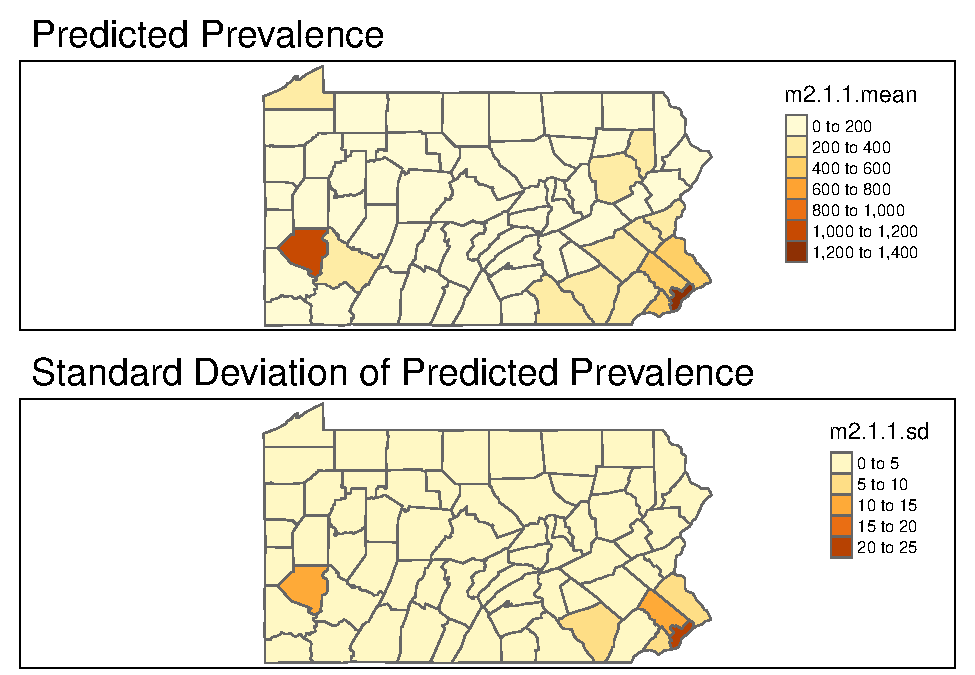
\includegraphics{hw4_files/figure-latex/unnamed-chunk-7-1.pdf}

\end{document}
